% Created 2017-10-24 Ter 13:54
\documentclass[11pt]{article}
\usepackage[utf8]{inputenc}
\usepackage[T1]{fontenc}
\usepackage{fixltx2e}
\usepackage{graphicx}
\usepackage{longtable}
\usepackage{float}
\usepackage{wrapfig}
\usepackage{rotating}
\usepackage[normalem]{ulem}
\usepackage{amsmath}
\usepackage{textcomp}
\usepackage{marvosym}
\usepackage{wasysym}
\usepackage{amssymb}
\usepackage{hyperref}
\tolerance=1000
\usepackage[margin=3cm]{geometry}
\author{Cecília Carneiro e Silva}
\date{25/10/2017}
\title{Trabalho 10}
\hypersetup{
  pdfkeywords={},
  pdfsubject={},
  pdfcreator={Emacs 25.1.1 (Org mode 8.2.10)}}
\begin{document}

\maketitle

\section{Trabalho 10 - Evolução diferencial}
\label{sec-1}

O objetivo desse trabalho é, usando evolução diferencial, minimizar a função de rosenbrock.

\begin{itemize}
\item Rosenbrock: f(x) = $\sum$[100 * (xi+i - xi²)² + (xi - 1)²]

\item Repositório do trabalho: \url{https://github.com/ceciliacsilva/deRosenbrock/}
\end{itemize}

\subsection{Configuração - DE}
\label{sec-1-1}

\begin{itemize}
\item np: tamanho da população;
\item cr: taxa de cruzamento;
\item f: constante (mutação);
\item xMin: x mínimo;
\item xMax: x máximo;
\item n: quantidade de 'x' no cromossomo;
\item endSimul: quantidade de gerações;
\item nRepeat: quantidade de vezes que caso o melhor individuo repita o algoritmo termina.
\end{itemize}

\subsection{Exemplos}
\label{sec-1-2}

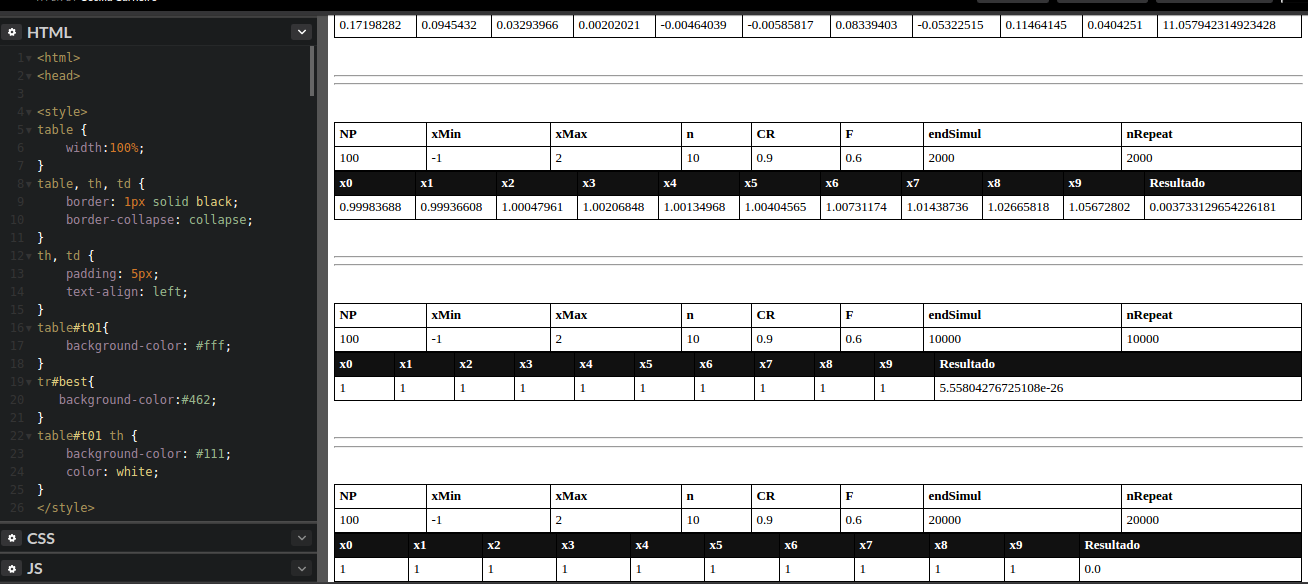
\includegraphics[width=.9\linewidth]{img/rosenbrock2.png}

Disponível em: \url{https://codepen.io/ceciliacsilva/pen/JrQbyM}

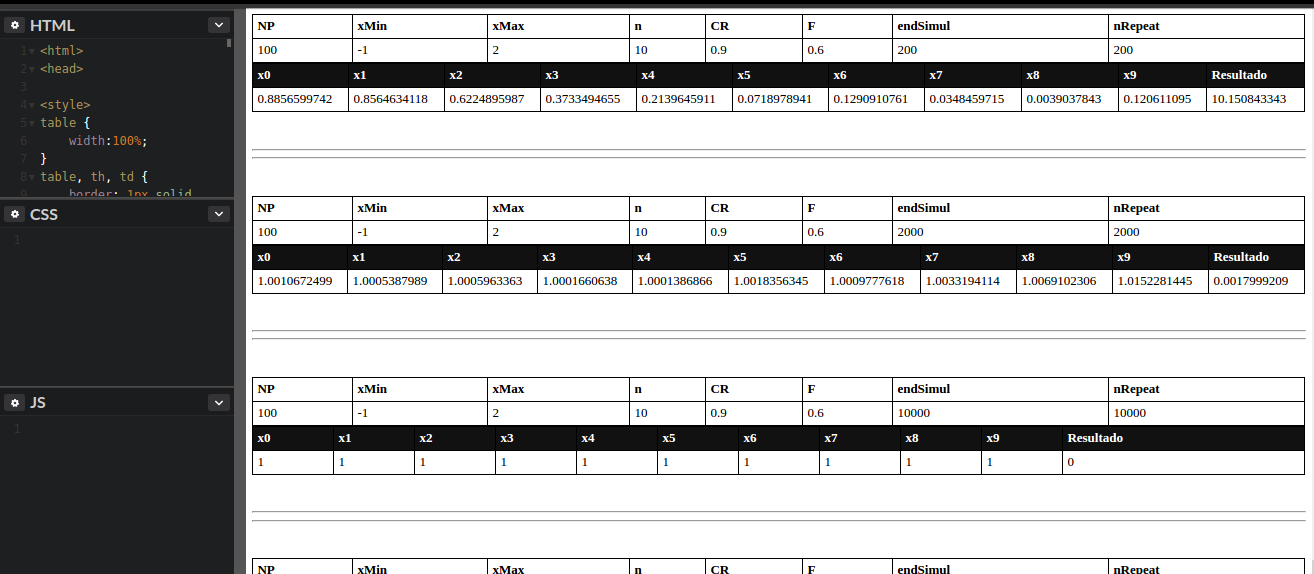
\includegraphics[width=.9\linewidth]{img/rosenbrock3.png}

Disponível em: \url{https://codepen.io/ceciliacsilva/pen/QqXGqb}
% Emacs 25.1.1 (Org mode 8.2.10)
\end{document}
